% Created by tikzDevice version 0.12.3.1 on 2022-05-02 11:32:14
% !TEX encoding = UTF-8 Unicode
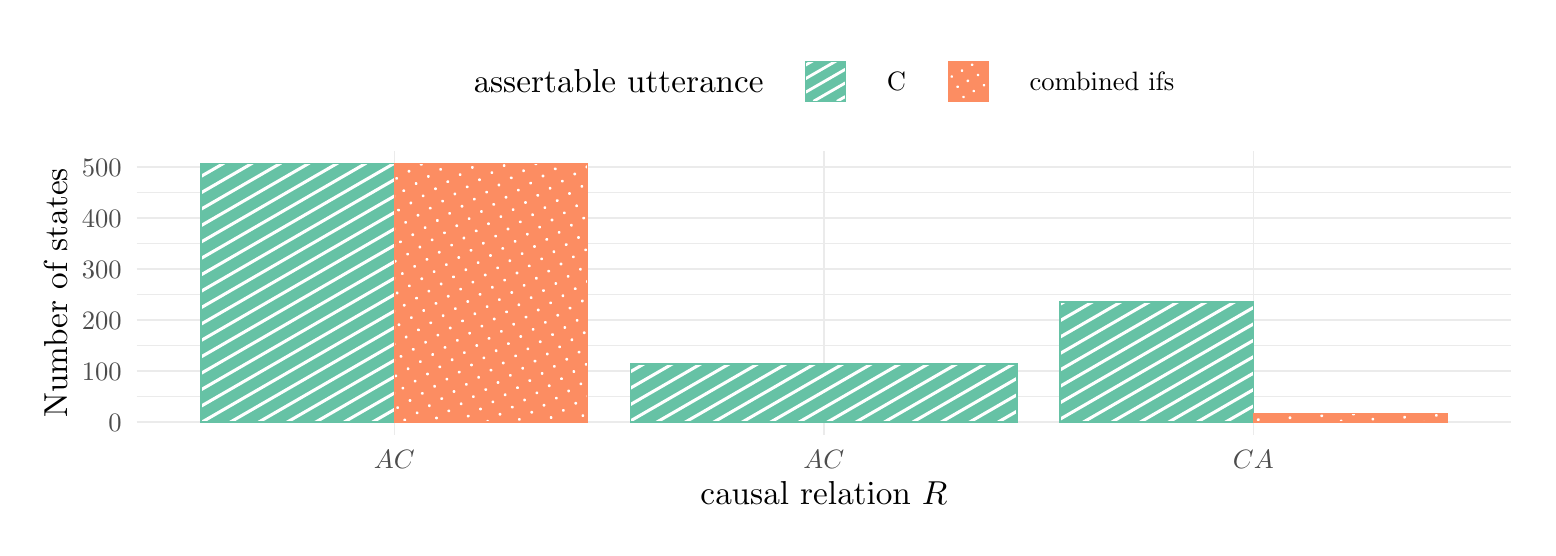
\begin{tikzpicture}[x=1pt,y=1pt]
\definecolor{fillColor}{RGB}{255,255,255}
\path[use as bounding box,fill=fillColor,fill opacity=0.00] (0,0) rectangle (542.02,180.67);
\begin{scope}
\path[clip] ( 39.39, 33.48) rectangle (536.02,136.22);
\definecolor{drawColor}{gray}{0.92}

\path[draw=drawColor,line width= 0.3pt,line join=round] ( 39.39, 47.36) --
	(536.02, 47.36);

\path[draw=drawColor,line width= 0.3pt,line join=round] ( 39.39, 65.78) --
	(536.02, 65.78);

\path[draw=drawColor,line width= 0.3pt,line join=round] ( 39.39, 84.20) --
	(536.02, 84.20);

\path[draw=drawColor,line width= 0.3pt,line join=round] ( 39.39,102.63) --
	(536.02,102.63);

\path[draw=drawColor,line width= 0.3pt,line join=round] ( 39.39,121.05) --
	(536.02,121.05);

\path[draw=drawColor,line width= 0.6pt,line join=round] ( 39.39, 38.15) --
	(536.02, 38.15);

\path[draw=drawColor,line width= 0.6pt,line join=round] ( 39.39, 56.57) --
	(536.02, 56.57);

\path[draw=drawColor,line width= 0.6pt,line join=round] ( 39.39, 74.99) --
	(536.02, 74.99);

\path[draw=drawColor,line width= 0.6pt,line join=round] ( 39.39, 93.41) --
	(536.02, 93.41);

\path[draw=drawColor,line width= 0.6pt,line join=round] ( 39.39,111.84) --
	(536.02,111.84);

\path[draw=drawColor,line width= 0.6pt,line join=round] ( 39.39,130.26) --
	(536.02,130.26);

\path[draw=drawColor,line width= 0.6pt,line join=round] (132.51, 33.48) --
	(132.51,136.22);

\path[draw=drawColor,line width= 0.6pt,line join=round] (287.71, 33.48) --
	(287.71,136.22);

\path[draw=drawColor,line width= 0.6pt,line join=round] (442.91, 33.48) --
	(442.91,136.22);
\definecolor{fillColor}{RGB}{102,194,165}

\path[fill=fillColor] ( 62.67, 38.15) rectangle (132.51,131.55);
\definecolor{fillColor}{RGB}{252,141,98}

\path[fill=fillColor] (132.51, 38.15) rectangle (202.35,131.55);
\definecolor{fillColor}{RGB}{102,194,165}

\path[fill=fillColor] (217.87, 38.15) rectangle (357.55, 59.15);

\path[fill=fillColor] (373.07, 38.15) rectangle (442.91, 81.44);
\definecolor{fillColor}{RGB}{252,141,98}

\path[fill=fillColor] (442.91, 38.15) rectangle (512.75, 41.28);
\definecolor{drawColor}{RGB}{255,255,255}
\definecolor{fillColor}{RGB}{255,255,255}

\path[draw=drawColor,line width= 0.6pt,line join=round,line cap=rect,fill=fillColor] (124.11, 38.15) --
	(132.51, 43.00) --
	(132.51, 42.40) --
	(125.14, 38.15) --
	(124.11, 38.15) --
	cycle;

\path[draw=drawColor,line width= 0.6pt,line join=round,line cap=rect,fill=fillColor] (113.83, 38.15) --
	(132.51, 48.93) --
	(132.51, 48.34) --
	(114.86, 38.15) --
	(113.83, 38.15) --
	cycle;

\path[draw=drawColor,line width= 0.6pt,line join=round,line cap=rect,fill=fillColor] (103.56, 38.15) --
	(132.51, 54.86) --
	(132.51, 54.27) --
	(104.59, 38.15) --
	(103.56, 38.15) --
	cycle;

\path[draw=drawColor,line width= 0.6pt,line join=round,line cap=rect,fill=fillColor] ( 93.28, 38.15) --
	(132.51, 60.79) --
	(132.51, 60.20) --
	( 94.31, 38.15) --
	( 93.28, 38.15) --
	cycle;

\path[draw=drawColor,line width= 0.6pt,line join=round,line cap=rect,fill=fillColor] ( 83.01, 38.15) --
	(132.51, 66.73) --
	(132.51, 66.13) --
	( 84.04, 38.15) --
	( 83.01, 38.15) --
	cycle;

\path[draw=drawColor,line width= 0.6pt,line join=round,line cap=rect,fill=fillColor] ( 72.74, 38.15) --
	(132.51, 72.66) --
	(132.51, 72.06) --
	( 73.76, 38.15) --
	( 72.74, 38.15) --
	cycle;

\path[draw=drawColor,line width= 0.6pt,line join=round,line cap=rect,fill=fillColor] ( 62.67, 38.27) --
	(132.51, 78.59) --
	(132.51, 78.00) --
	( 63.49, 38.15) --
	( 62.67, 38.15) --
	( 62.67, 38.27) --
	cycle;

\path[draw=drawColor,line width= 0.6pt,line join=round,line cap=rect,fill=fillColor] ( 62.67, 44.20) --
	(132.51, 84.52) --
	(132.51, 83.93) --
	( 62.67, 43.61) --
	( 62.67, 44.20) --
	cycle;

\path[draw=drawColor,line width= 0.6pt,line join=round,line cap=rect,fill=fillColor] ( 62.67, 50.13) --
	(132.51, 90.45) --
	(132.51, 89.86) --
	( 62.67, 49.54) --
	( 62.67, 50.13) --
	cycle;

\path[draw=drawColor,line width= 0.6pt,line join=round,line cap=rect,fill=fillColor] ( 62.67, 56.06) --
	(132.51, 96.39) --
	(132.51, 95.79) --
	( 62.67, 55.47) --
	( 62.67, 56.06) --
	cycle;

\path[draw=drawColor,line width= 0.6pt,line join=round,line cap=rect,fill=fillColor] ( 62.67, 62.00) --
	(132.51,102.32) --
	(132.51,101.72) --
	( 62.67, 61.40) --
	( 62.67, 62.00) --
	cycle;

\path[draw=drawColor,line width= 0.6pt,line join=round,line cap=rect,fill=fillColor] ( 62.67, 67.93) --
	(132.51,108.25) --
	(132.51,107.66) --
	( 62.67, 67.34) --
	( 62.67, 67.93) --
	cycle;

\path[draw=drawColor,line width= 0.6pt,line join=round,line cap=rect,fill=fillColor] ( 62.67, 73.86) --
	(132.51,114.18) --
	(132.51,113.59) --
	( 62.67, 73.27) --
	( 62.67, 73.86) --
	cycle;

\path[draw=drawColor,line width= 0.6pt,line join=round,line cap=rect,fill=fillColor] ( 62.67, 79.79) --
	(132.51,120.11) --
	(132.51,119.52) --
	( 62.67, 79.20) --
	( 62.67, 79.79) --
	cycle;

\path[draw=drawColor,line width= 0.6pt,line join=round,line cap=rect,fill=fillColor] ( 62.67, 85.72) --
	(132.51,126.05) --
	(132.51,125.45) --
	( 62.67, 85.13) --
	( 62.67, 85.72) --
	cycle;

\path[draw=drawColor,line width= 0.6pt,line join=round,line cap=rect,fill=fillColor] ( 62.67, 91.66) --
	(131.77,131.55) --
	(132.51,131.55) --
	(132.51,131.38) --
	( 62.67, 91.06) --
	( 62.67, 91.66) --
	cycle;

\path[draw=drawColor,line width= 0.6pt,line join=round,line cap=rect,fill=fillColor] ( 62.67, 97.59) --
	(121.50,131.55) --
	(122.52,131.55) --
	( 62.67, 97.00) --
	( 62.67, 97.59) --
	cycle;

\path[draw=drawColor,line width= 0.6pt,line join=round,line cap=rect,fill=fillColor] ( 62.67,103.52) --
	(111.22,131.55) --
	(112.25,131.55) --
	( 62.67,102.93) --
	( 62.67,103.52) --
	cycle;

\path[draw=drawColor,line width= 0.6pt,line join=round,line cap=rect,fill=fillColor] ( 62.67,109.45) --
	(100.95,131.55) --
	(101.98,131.55) --
	( 62.67,108.86) --
	( 62.67,109.45) --
	cycle;

\path[draw=drawColor,line width= 0.6pt,line join=round,line cap=rect,fill=fillColor] ( 62.67,115.38) --
	( 90.67,131.55) --
	( 91.70,131.55) --
	( 62.67,114.79) --
	( 62.67,115.38) --
	cycle;

\path[draw=drawColor,line width= 0.6pt,line join=round,line cap=rect,fill=fillColor] ( 62.67,121.32) --
	( 80.40,131.55) --
	( 81.43,131.55) --
	( 62.67,120.72) --
	( 62.67,121.32) --
	cycle;

\path[draw=drawColor,line width= 0.6pt,line join=round,line cap=rect,fill=fillColor] ( 62.67,127.25) --
	( 70.12,131.55) --
	( 71.15,131.55) --
	( 62.67,126.66) --
	( 62.67,127.25) --
	cycle;

\path[draw=drawColor,line width= 0.6pt,dash pattern=on 2pt off 2pt ,line join=round,line cap=round,fill=fillColor] (132.82, 96.27) circle (  0.26);

\path[draw=drawColor,line width= 0.6pt,dash pattern=on 2pt off 2pt ,line join=round,line cap=round,fill=fillColor] (133.00, 54.85) circle (  0.26);

\path[draw=drawColor,line width= 0.6pt,dash pattern=on 2pt off 2pt ,line join=round,line cap=round,fill=fillColor] (133.32,126.22) circle (  0.26);

\path[draw=drawColor,line width= 0.6pt,dash pattern=on 2pt off 2pt ,line join=round,line cap=round,fill=fillColor] (133.51, 84.80) circle (  0.26);

\path[draw=drawColor,line width= 0.6pt,dash pattern=on 2pt off 2pt ,line join=round,line cap=round,fill=fillColor] (133.69, 43.38) circle (  0.26);

\path[draw=drawColor,line width= 0.6pt,dash pattern=on 2pt off 2pt ,line join=round,line cap=round,fill=fillColor] (134.01,114.75) circle (  0.26);

\path[draw=drawColor,line width= 0.6pt,dash pattern=on 2pt off 2pt ,line join=round,line cap=round,fill=fillColor] (134.19, 73.33) circle (  0.26);

\path[draw=drawColor,line width= 0.6pt,dash pattern=on 2pt off 2pt ,line join=round,line cap=round,fill=fillColor] (134.70,103.28) circle (  0.26);

\path[draw=drawColor,line width= 0.6pt,dash pattern=on 2pt off 2pt ,line join=round,line cap=round,fill=fillColor] (134.88, 61.87) circle (  0.26);

\path[draw=drawColor,line width= 0.6pt,dash pattern=on 2pt off 2pt ,line join=round,line cap=round,fill=fillColor] (135.39, 91.82) circle (  0.26);

\path[draw=drawColor,line width= 0.6pt,dash pattern=on 2pt off 2pt ,line join=round,line cap=round,fill=fillColor] (135.57, 50.40) circle (  0.26);

\path[draw=drawColor,line width= 0.6pt,dash pattern=on 2pt off 2pt ,line join=round,line cap=round,fill=fillColor] (135.89,121.77) circle (  0.26);

\path[draw=drawColor,line width= 0.6pt,dash pattern=on 2pt off 2pt ,line join=round,line cap=round,fill=fillColor] (136.07, 80.35) circle (  0.26);

\path[draw=drawColor,line width= 0.6pt,dash pattern=on 2pt off 2pt ,line join=round,line cap=round,fill=fillColor] (136.26, 38.93) circle (  0.26);

\path[draw=drawColor,line width= 0.6pt,dash pattern=on 2pt off 2pt ,line join=round,line cap=round,fill=fillColor] (136.58,110.30) circle (  0.26);

\path[draw=drawColor,line width= 0.6pt,dash pattern=on 2pt off 2pt ,line join=round,line cap=round,fill=fillColor] (136.76, 68.88) circle (  0.26);

\path[draw=drawColor,line width= 0.6pt,dash pattern=on 2pt off 2pt ,line join=round,line cap=round,fill=fillColor] (137.27, 98.83) circle (  0.26);

\path[draw=drawColor,line width= 0.6pt,dash pattern=on 2pt off 2pt ,line join=round,line cap=round,fill=fillColor] (137.45, 57.42) circle (  0.26);

\path[draw=drawColor,line width= 0.6pt,dash pattern=on 2pt off 2pt ,line join=round,line cap=round,fill=fillColor] (137.77,128.79) circle (  0.26);

\path[draw=drawColor,line width= 0.6pt,dash pattern=on 2pt off 2pt ,line join=round,line cap=round,fill=fillColor] (137.95, 87.37) circle (  0.26);

\path[draw=drawColor,line width= 0.6pt,dash pattern=on 2pt off 2pt ,line join=round,line cap=round,fill=fillColor] (138.14, 45.95) circle (  0.26);

\path[draw=drawColor,line width= 0.6pt,dash pattern=on 2pt off 2pt ,line join=round,line cap=round,fill=fillColor] (138.46,117.32) circle (  0.26);

\path[draw=drawColor,line width= 0.6pt,dash pattern=on 2pt off 2pt ,line join=round,line cap=round,fill=fillColor] (138.64, 75.90) circle (  0.26);

\path[draw=drawColor,line width= 0.6pt,dash pattern=on 2pt off 2pt ,line join=round,line cap=round,fill=fillColor] (139.15,105.85) circle (  0.26);

\path[draw=drawColor,line width= 0.6pt,dash pattern=on 2pt off 2pt ,line join=round,line cap=round,fill=fillColor] (139.33, 64.43) circle (  0.26);

\path[draw=drawColor,line width= 0.6pt,dash pattern=on 2pt off 2pt ,line join=round,line cap=round,fill=fillColor] (139.83, 94.39) circle (  0.26);

\path[draw=drawColor,line width= 0.6pt,dash pattern=on 2pt off 2pt ,line join=round,line cap=round,fill=fillColor] (140.02, 52.97) circle (  0.26);

\path[draw=drawColor,line width= 0.6pt,dash pattern=on 2pt off 2pt ,line join=round,line cap=round,fill=fillColor] (140.34,124.34) circle (  0.26);

\path[draw=drawColor,line width= 0.6pt,dash pattern=on 2pt off 2pt ,line join=round,line cap=round,fill=fillColor] (140.52, 82.92) circle (  0.26);

\path[draw=drawColor,line width= 0.6pt,dash pattern=on 2pt off 2pt ,line join=round,line cap=round,fill=fillColor] (140.71, 41.50) circle (  0.26);

\path[draw=drawColor,line width= 0.6pt,dash pattern=on 2pt off 2pt ,line join=round,line cap=round,fill=fillColor] (141.03,112.87) circle (  0.26);

\path[draw=drawColor,line width= 0.6pt,dash pattern=on 2pt off 2pt ,line join=round,line cap=round,fill=fillColor] (141.21, 71.45) circle (  0.26);

\path[draw=drawColor,line width= 0.6pt,dash pattern=on 2pt off 2pt ,line join=round,line cap=round,fill=fillColor] (141.72,101.40) circle (  0.26);

\path[draw=drawColor,line width= 0.6pt,dash pattern=on 2pt off 2pt ,line join=round,line cap=round,fill=fillColor] (141.90, 59.99) circle (  0.26);

\path[draw=drawColor,line width= 0.6pt,dash pattern=on 2pt off 2pt ,line join=round,line cap=round,fill=fillColor] (142.40, 89.94) circle (  0.26);

\path[draw=drawColor,line width= 0.6pt,dash pattern=on 2pt off 2pt ,line join=round,line cap=round,fill=fillColor] (142.59, 48.52) circle (  0.26);

\path[draw=drawColor,line width= 0.6pt,dash pattern=on 2pt off 2pt ,line join=round,line cap=round,fill=fillColor] (142.91,119.89) circle (  0.26);

\path[draw=drawColor,line width= 0.6pt,dash pattern=on 2pt off 2pt ,line join=round,line cap=round,fill=fillColor] (143.09, 78.47) circle (  0.26);

\path[draw=drawColor,line width= 0.6pt,dash pattern=on 2pt off 2pt ,line join=round,line cap=round,fill=fillColor] (143.60,108.42) circle (  0.26);

\path[draw=drawColor,line width= 0.6pt,dash pattern=on 2pt off 2pt ,line join=round,line cap=round,fill=fillColor] (143.78, 67.00) circle (  0.26);

\path[draw=drawColor,line width= 0.6pt,dash pattern=on 2pt off 2pt ,line join=round,line cap=round,fill=fillColor] (144.28, 96.95) circle (  0.26);

\path[draw=drawColor,line width= 0.6pt,dash pattern=on 2pt off 2pt ,line join=round,line cap=round,fill=fillColor] (144.47, 55.54) circle (  0.26);

\path[draw=drawColor,line width= 0.6pt,dash pattern=on 2pt off 2pt ,line join=round,line cap=round,fill=fillColor] (144.79,126.90) circle (  0.26);

\path[draw=drawColor,line width= 0.6pt,dash pattern=on 2pt off 2pt ,line join=round,line cap=round,fill=fillColor] (144.97, 85.49) circle (  0.26);

\path[draw=drawColor,line width= 0.6pt,dash pattern=on 2pt off 2pt ,line join=round,line cap=round,fill=fillColor] (145.16, 44.07) circle (  0.26);

\path[draw=drawColor,line width= 0.6pt,dash pattern=on 2pt off 2pt ,line join=round,line cap=round,fill=fillColor] (145.48,115.44) circle (  0.26);

\path[draw=drawColor,line width= 0.6pt,dash pattern=on 2pt off 2pt ,line join=round,line cap=round,fill=fillColor] (145.66, 74.02) circle (  0.26);

\path[draw=drawColor,line width= 0.6pt,dash pattern=on 2pt off 2pt ,line join=round,line cap=round,fill=fillColor] (146.16,103.97) circle (  0.26);

\path[draw=drawColor,line width= 0.6pt,dash pattern=on 2pt off 2pt ,line join=round,line cap=round,fill=fillColor] (146.35, 62.55) circle (  0.26);

\path[draw=drawColor,line width= 0.6pt,dash pattern=on 2pt off 2pt ,line join=round,line cap=round,fill=fillColor] (146.85, 92.50) circle (  0.26);

\path[draw=drawColor,line width= 0.6pt,dash pattern=on 2pt off 2pt ,line join=round,line cap=round,fill=fillColor] (147.04, 51.09) circle (  0.26);

\path[draw=drawColor,line width= 0.6pt,dash pattern=on 2pt off 2pt ,line join=round,line cap=round,fill=fillColor] (147.36,122.46) circle (  0.26);

\path[draw=drawColor,line width= 0.6pt,dash pattern=on 2pt off 2pt ,line join=round,line cap=round,fill=fillColor] (147.54, 81.04) circle (  0.26);

\path[draw=drawColor,line width= 0.6pt,dash pattern=on 2pt off 2pt ,line join=round,line cap=round,fill=fillColor] (147.73, 39.62) circle (  0.26);

\path[draw=drawColor,line width= 0.6pt,dash pattern=on 2pt off 2pt ,line join=round,line cap=round,fill=fillColor] (148.04,110.99) circle (  0.26);

\path[draw=drawColor,line width= 0.6pt,dash pattern=on 2pt off 2pt ,line join=round,line cap=round,fill=fillColor] (148.23, 69.57) circle (  0.26);

\path[draw=drawColor,line width= 0.6pt,dash pattern=on 2pt off 2pt ,line join=round,line cap=round,fill=fillColor] (148.73, 99.52) circle (  0.26);

\path[draw=drawColor,line width= 0.6pt,dash pattern=on 2pt off 2pt ,line join=round,line cap=round,fill=fillColor] (148.92, 58.10) circle (  0.26);

\path[draw=drawColor,line width= 0.6pt,dash pattern=on 2pt off 2pt ,line join=round,line cap=round,fill=fillColor] (149.24,129.47) circle (  0.26);

\path[draw=drawColor,line width= 0.6pt,dash pattern=on 2pt off 2pt ,line join=round,line cap=round,fill=fillColor] (149.42, 88.06) circle (  0.26);

\path[draw=drawColor,line width= 0.6pt,dash pattern=on 2pt off 2pt ,line join=round,line cap=round,fill=fillColor] (149.61, 46.64) circle (  0.26);

\path[draw=drawColor,line width= 0.6pt,dash pattern=on 2pt off 2pt ,line join=round,line cap=round,fill=fillColor] (149.92,118.01) circle (  0.26);

\path[draw=drawColor,line width= 0.6pt,dash pattern=on 2pt off 2pt ,line join=round,line cap=round,fill=fillColor] (150.11, 76.59) circle (  0.26);

\path[draw=drawColor,line width= 0.6pt,dash pattern=on 2pt off 2pt ,line join=round,line cap=round,fill=fillColor] (150.61,106.54) circle (  0.26);

\path[draw=drawColor,line width= 0.6pt,dash pattern=on 2pt off 2pt ,line join=round,line cap=round,fill=fillColor] (150.80, 65.12) circle (  0.26);

\path[draw=drawColor,line width= 0.6pt,dash pattern=on 2pt off 2pt ,line join=round,line cap=round,fill=fillColor] (151.30, 95.07) circle (  0.26);

\path[draw=drawColor,line width= 0.6pt,dash pattern=on 2pt off 2pt ,line join=round,line cap=round,fill=fillColor] (151.49, 53.66) circle (  0.26);

\path[draw=drawColor,line width= 0.6pt,dash pattern=on 2pt off 2pt ,line join=round,line cap=round,fill=fillColor] (151.81,125.02) circle (  0.26);

\path[draw=drawColor,line width= 0.6pt,dash pattern=on 2pt off 2pt ,line join=round,line cap=round,fill=fillColor] (151.99, 83.61) circle (  0.26);

\path[draw=drawColor,line width= 0.6pt,dash pattern=on 2pt off 2pt ,line join=round,line cap=round,fill=fillColor] (152.17, 42.19) circle (  0.26);

\path[draw=drawColor,line width= 0.6pt,dash pattern=on 2pt off 2pt ,line join=round,line cap=round,fill=fillColor] (152.49,113.56) circle (  0.26);

\path[draw=drawColor,line width= 0.6pt,dash pattern=on 2pt off 2pt ,line join=round,line cap=round,fill=fillColor] (152.68, 72.14) circle (  0.26);

\path[draw=drawColor,line width= 0.6pt,dash pattern=on 2pt off 2pt ,line join=round,line cap=round,fill=fillColor] (153.18,102.09) circle (  0.26);

\path[draw=drawColor,line width= 0.6pt,dash pattern=on 2pt off 2pt ,line join=round,line cap=round,fill=fillColor] (153.37, 60.67) circle (  0.26);

\path[draw=drawColor,line width= 0.6pt,dash pattern=on 2pt off 2pt ,line join=round,line cap=round,fill=fillColor] (153.87, 90.62) circle (  0.26);

\path[draw=drawColor,line width= 0.6pt,dash pattern=on 2pt off 2pt ,line join=round,line cap=round,fill=fillColor] (154.05, 49.21) circle (  0.26);

\path[draw=drawColor,line width= 0.6pt,dash pattern=on 2pt off 2pt ,line join=round,line cap=round,fill=fillColor] (154.37,120.58) circle (  0.26);

\path[draw=drawColor,line width= 0.6pt,dash pattern=on 2pt off 2pt ,line join=round,line cap=round,fill=fillColor] (154.56, 79.16) circle (  0.26);

\path[draw=drawColor,line width= 0.6pt,dash pattern=on 2pt off 2pt ,line join=round,line cap=round,fill=fillColor] (155.06,109.11) circle (  0.26);

\path[draw=drawColor,line width= 0.6pt,dash pattern=on 2pt off 2pt ,line join=round,line cap=round,fill=fillColor] (155.25, 67.69) circle (  0.26);

\path[draw=drawColor,line width= 0.6pt,dash pattern=on 2pt off 2pt ,line join=round,line cap=round,fill=fillColor] (155.75, 97.64) circle (  0.26);

\path[draw=drawColor,line width= 0.6pt,dash pattern=on 2pt off 2pt ,line join=round,line cap=round,fill=fillColor] (155.93, 56.22) circle (  0.26);

\path[draw=drawColor,line width= 0.6pt,dash pattern=on 2pt off 2pt ,line join=round,line cap=round,fill=fillColor] (156.25,127.59) circle (  0.26);

\path[draw=drawColor,line width= 0.6pt,dash pattern=on 2pt off 2pt ,line join=round,line cap=round,fill=fillColor] (156.44, 86.18) circle (  0.26);

\path[draw=drawColor,line width= 0.6pt,dash pattern=on 2pt off 2pt ,line join=round,line cap=round,fill=fillColor] (156.62, 44.76) circle (  0.26);

\path[draw=drawColor,line width= 0.6pt,dash pattern=on 2pt off 2pt ,line join=round,line cap=round,fill=fillColor] (156.94,116.13) circle (  0.26);

\path[draw=drawColor,line width= 0.6pt,dash pattern=on 2pt off 2pt ,line join=round,line cap=round,fill=fillColor] (157.13, 74.71) circle (  0.26);

\path[draw=drawColor,line width= 0.6pt,dash pattern=on 2pt off 2pt ,line join=round,line cap=round,fill=fillColor] (157.63,104.66) circle (  0.26);

\path[draw=drawColor,line width= 0.6pt,dash pattern=on 2pt off 2pt ,line join=round,line cap=round,fill=fillColor] (157.82, 63.24) circle (  0.26);

\path[draw=drawColor,line width= 0.6pt,dash pattern=on 2pt off 2pt ,line join=round,line cap=round,fill=fillColor] (158.32, 93.19) circle (  0.26);

\path[draw=drawColor,line width= 0.6pt,dash pattern=on 2pt off 2pt ,line join=round,line cap=round,fill=fillColor] (158.50, 51.78) circle (  0.26);

\path[draw=drawColor,line width= 0.6pt,dash pattern=on 2pt off 2pt ,line join=round,line cap=round,fill=fillColor] (158.82,123.14) circle (  0.26);

\path[draw=drawColor,line width= 0.6pt,dash pattern=on 2pt off 2pt ,line join=round,line cap=round,fill=fillColor] (159.01, 81.73) circle (  0.26);

\path[draw=drawColor,line width= 0.6pt,dash pattern=on 2pt off 2pt ,line join=round,line cap=round,fill=fillColor] (159.19, 40.31) circle (  0.26);

\path[draw=drawColor,line width= 0.6pt,dash pattern=on 2pt off 2pt ,line join=round,line cap=round,fill=fillColor] (159.51,111.68) circle (  0.26);

\path[draw=drawColor,line width= 0.6pt,dash pattern=on 2pt off 2pt ,line join=round,line cap=round,fill=fillColor] (159.70, 70.26) circle (  0.26);

\path[draw=drawColor,line width= 0.6pt,dash pattern=on 2pt off 2pt ,line join=round,line cap=round,fill=fillColor] (160.20,100.21) circle (  0.26);

\path[draw=drawColor,line width= 0.6pt,dash pattern=on 2pt off 2pt ,line join=round,line cap=round,fill=fillColor] (160.38, 58.79) circle (  0.26);

\path[draw=drawColor,line width= 0.6pt,dash pattern=on 2pt off 2pt ,line join=round,line cap=round,fill=fillColor] (160.70,130.16) circle (  0.26);

\path[draw=drawColor,line width= 0.6pt,dash pattern=on 2pt off 2pt ,line join=round,line cap=round,fill=fillColor] (160.89, 88.74) circle (  0.26);

\path[draw=drawColor,line width= 0.6pt,dash pattern=on 2pt off 2pt ,line join=round,line cap=round,fill=fillColor] (161.07, 47.33) circle (  0.26);

\path[draw=drawColor,line width= 0.6pt,dash pattern=on 2pt off 2pt ,line join=round,line cap=round,fill=fillColor] (161.39,118.69) circle (  0.26);

\path[draw=drawColor,line width= 0.6pt,dash pattern=on 2pt off 2pt ,line join=round,line cap=round,fill=fillColor] (161.58, 77.28) circle (  0.26);

\path[draw=drawColor,line width= 0.6pt,dash pattern=on 2pt off 2pt ,line join=round,line cap=round,fill=fillColor] (162.08,107.23) circle (  0.26);

\path[draw=drawColor,line width= 0.6pt,dash pattern=on 2pt off 2pt ,line join=round,line cap=round,fill=fillColor] (162.26, 65.81) circle (  0.26);

\path[draw=drawColor,line width= 0.6pt,dash pattern=on 2pt off 2pt ,line join=round,line cap=round,fill=fillColor] (162.77, 95.76) circle (  0.26);

\path[draw=drawColor,line width= 0.6pt,dash pattern=on 2pt off 2pt ,line join=round,line cap=round,fill=fillColor] (162.95, 54.34) circle (  0.26);

\path[draw=drawColor,line width= 0.6pt,dash pattern=on 2pt off 2pt ,line join=round,line cap=round,fill=fillColor] (163.27,125.71) circle (  0.26);

\path[draw=drawColor,line width= 0.6pt,dash pattern=on 2pt off 2pt ,line join=round,line cap=round,fill=fillColor] (163.46, 84.29) circle (  0.26);

\path[draw=drawColor,line width= 0.6pt,dash pattern=on 2pt off 2pt ,line join=round,line cap=round,fill=fillColor] (163.64, 42.88) circle (  0.26);

\path[draw=drawColor,line width= 0.6pt,dash pattern=on 2pt off 2pt ,line join=round,line cap=round,fill=fillColor] (163.96,114.25) circle (  0.26);

\path[draw=drawColor,line width= 0.6pt,dash pattern=on 2pt off 2pt ,line join=round,line cap=round,fill=fillColor] (164.14, 72.83) circle (  0.26);

\path[draw=drawColor,line width= 0.6pt,dash pattern=on 2pt off 2pt ,line join=round,line cap=round,fill=fillColor] (164.65,102.78) circle (  0.26);

\path[draw=drawColor,line width= 0.6pt,dash pattern=on 2pt off 2pt ,line join=round,line cap=round,fill=fillColor] (164.83, 61.36) circle (  0.26);

\path[draw=drawColor,line width= 0.6pt,dash pattern=on 2pt off 2pt ,line join=round,line cap=round,fill=fillColor] (165.34, 91.31) circle (  0.26);

\path[draw=drawColor,line width= 0.6pt,dash pattern=on 2pt off 2pt ,line join=round,line cap=round,fill=fillColor] (165.52, 49.89) circle (  0.26);

\path[draw=drawColor,line width= 0.6pt,dash pattern=on 2pt off 2pt ,line join=round,line cap=round,fill=fillColor] (165.84,121.26) circle (  0.26);

\path[draw=drawColor,line width= 0.6pt,dash pattern=on 2pt off 2pt ,line join=round,line cap=round,fill=fillColor] (166.03, 79.85) circle (  0.26);

\path[draw=drawColor,line width= 0.6pt,dash pattern=on 2pt off 2pt ,line join=round,line cap=round,fill=fillColor] (166.21, 38.43) circle (  0.26);

\path[draw=drawColor,line width= 0.6pt,dash pattern=on 2pt off 2pt ,line join=round,line cap=round,fill=fillColor] (166.53,109.80) circle (  0.26);

\path[draw=drawColor,line width= 0.6pt,dash pattern=on 2pt off 2pt ,line join=round,line cap=round,fill=fillColor] (166.71, 68.38) circle (  0.26);

\path[draw=drawColor,line width= 0.6pt,dash pattern=on 2pt off 2pt ,line join=round,line cap=round,fill=fillColor] (167.22, 98.33) circle (  0.26);

\path[draw=drawColor,line width= 0.6pt,dash pattern=on 2pt off 2pt ,line join=round,line cap=round,fill=fillColor] (167.40, 56.91) circle (  0.26);

\path[draw=drawColor,line width= 0.6pt,dash pattern=on 2pt off 2pt ,line join=round,line cap=round,fill=fillColor] (167.72,128.28) circle (  0.26);

\path[draw=drawColor,line width= 0.6pt,dash pattern=on 2pt off 2pt ,line join=round,line cap=round,fill=fillColor] (167.91, 86.86) circle (  0.26);

\path[draw=drawColor,line width= 0.6pt,dash pattern=on 2pt off 2pt ,line join=round,line cap=round,fill=fillColor] (168.09, 45.45) circle (  0.26);

\path[draw=drawColor,line width= 0.6pt,dash pattern=on 2pt off 2pt ,line join=round,line cap=round,fill=fillColor] (168.41,116.81) circle (  0.26);

\path[draw=drawColor,line width= 0.6pt,dash pattern=on 2pt off 2pt ,line join=round,line cap=round,fill=fillColor] (168.59, 75.40) circle (  0.26);

\path[draw=drawColor,line width= 0.6pt,dash pattern=on 2pt off 2pt ,line join=round,line cap=round,fill=fillColor] (169.10,105.35) circle (  0.26);

\path[draw=drawColor,line width= 0.6pt,dash pattern=on 2pt off 2pt ,line join=round,line cap=round,fill=fillColor] (169.28, 63.93) circle (  0.26);

\path[draw=drawColor,line width= 0.6pt,dash pattern=on 2pt off 2pt ,line join=round,line cap=round,fill=fillColor] (169.79, 93.88) circle (  0.26);

\path[draw=drawColor,line width= 0.6pt,dash pattern=on 2pt off 2pt ,line join=round,line cap=round,fill=fillColor] (169.97, 52.46) circle (  0.26);

\path[draw=drawColor,line width= 0.6pt,dash pattern=on 2pt off 2pt ,line join=round,line cap=round,fill=fillColor] (170.29,123.83) circle (  0.26);

\path[draw=drawColor,line width= 0.6pt,dash pattern=on 2pt off 2pt ,line join=round,line cap=round,fill=fillColor] (170.47, 82.41) circle (  0.26);

\path[draw=drawColor,line width= 0.6pt,dash pattern=on 2pt off 2pt ,line join=round,line cap=round,fill=fillColor] (170.66, 41.00) circle (  0.26);

\path[draw=drawColor,line width= 0.6pt,dash pattern=on 2pt off 2pt ,line join=round,line cap=round,fill=fillColor] (170.98,112.37) circle (  0.26);

\path[draw=drawColor,line width= 0.6pt,dash pattern=on 2pt off 2pt ,line join=round,line cap=round,fill=fillColor] (171.16, 70.95) circle (  0.26);

\path[draw=drawColor,line width= 0.6pt,dash pattern=on 2pt off 2pt ,line join=round,line cap=round,fill=fillColor] (171.67,100.90) circle (  0.26);

\path[draw=drawColor,line width= 0.6pt,dash pattern=on 2pt off 2pt ,line join=round,line cap=round,fill=fillColor] (171.85, 59.48) circle (  0.26);

\path[draw=drawColor,line width= 0.6pt,dash pattern=on 2pt off 2pt ,line join=round,line cap=round,fill=fillColor] (172.17,130.85) circle (  0.26);

\path[draw=drawColor,line width= 0.6pt,dash pattern=on 2pt off 2pt ,line join=round,line cap=round,fill=fillColor] (172.35, 89.43) circle (  0.26);

\path[draw=drawColor,line width= 0.6pt,dash pattern=on 2pt off 2pt ,line join=round,line cap=round,fill=fillColor] (172.54, 48.01) circle (  0.26);

\path[draw=drawColor,line width= 0.6pt,dash pattern=on 2pt off 2pt ,line join=round,line cap=round,fill=fillColor] (172.86,119.38) circle (  0.26);

\path[draw=drawColor,line width= 0.6pt,dash pattern=on 2pt off 2pt ,line join=round,line cap=round,fill=fillColor] (173.04, 77.97) circle (  0.26);

\path[draw=drawColor,line width= 0.6pt,dash pattern=on 2pt off 2pt ,line join=round,line cap=round,fill=fillColor] (173.55,107.92) circle (  0.26);

\path[draw=drawColor,line width= 0.6pt,dash pattern=on 2pt off 2pt ,line join=round,line cap=round,fill=fillColor] (173.73, 66.50) circle (  0.26);

\path[draw=drawColor,line width= 0.6pt,dash pattern=on 2pt off 2pt ,line join=round,line cap=round,fill=fillColor] (174.23, 96.45) circle (  0.26);

\path[draw=drawColor,line width= 0.6pt,dash pattern=on 2pt off 2pt ,line join=round,line cap=round,fill=fillColor] (174.42, 55.03) circle (  0.26);

\path[draw=drawColor,line width= 0.6pt,dash pattern=on 2pt off 2pt ,line join=round,line cap=round,fill=fillColor] (174.74,126.40) circle (  0.26);

\path[draw=drawColor,line width= 0.6pt,dash pattern=on 2pt off 2pt ,line join=round,line cap=round,fill=fillColor] (174.92, 84.98) circle (  0.26);

\path[draw=drawColor,line width= 0.6pt,dash pattern=on 2pt off 2pt ,line join=round,line cap=round,fill=fillColor] (175.11, 43.57) circle (  0.26);

\path[draw=drawColor,line width= 0.6pt,dash pattern=on 2pt off 2pt ,line join=round,line cap=round,fill=fillColor] (175.43,114.93) circle (  0.26);

\path[draw=drawColor,line width= 0.6pt,dash pattern=on 2pt off 2pt ,line join=round,line cap=round,fill=fillColor] (175.61, 73.52) circle (  0.26);

\path[draw=drawColor,line width= 0.6pt,dash pattern=on 2pt off 2pt ,line join=round,line cap=round,fill=fillColor] (176.12,103.47) circle (  0.26);

\path[draw=drawColor,line width= 0.6pt,dash pattern=on 2pt off 2pt ,line join=round,line cap=round,fill=fillColor] (176.30, 62.05) circle (  0.26);

\path[draw=drawColor,line width= 0.6pt,dash pattern=on 2pt off 2pt ,line join=round,line cap=round,fill=fillColor] (176.80, 92.00) circle (  0.26);

\path[draw=drawColor,line width= 0.6pt,dash pattern=on 2pt off 2pt ,line join=round,line cap=round,fill=fillColor] (176.99, 50.58) circle (  0.26);

\path[draw=drawColor,line width= 0.6pt,dash pattern=on 2pt off 2pt ,line join=round,line cap=round,fill=fillColor] (177.31,121.95) circle (  0.26);

\path[draw=drawColor,line width= 0.6pt,dash pattern=on 2pt off 2pt ,line join=round,line cap=round,fill=fillColor] (177.49, 80.53) circle (  0.26);

\path[draw=drawColor,line width= 0.6pt,dash pattern=on 2pt off 2pt ,line join=round,line cap=round,fill=fillColor] (177.68, 39.12) circle (  0.26);

\path[draw=drawColor,line width= 0.6pt,dash pattern=on 2pt off 2pt ,line join=round,line cap=round,fill=fillColor] (178.00,110.49) circle (  0.26);

\path[draw=drawColor,line width= 0.6pt,dash pattern=on 2pt off 2pt ,line join=round,line cap=round,fill=fillColor] (178.18, 69.07) circle (  0.26);

\path[draw=drawColor,line width= 0.6pt,dash pattern=on 2pt off 2pt ,line join=round,line cap=round,fill=fillColor] (178.68, 99.02) circle (  0.26);

\path[draw=drawColor,line width= 0.6pt,dash pattern=on 2pt off 2pt ,line join=round,line cap=round,fill=fillColor] (178.87, 57.60) circle (  0.26);

\path[draw=drawColor,line width= 0.6pt,dash pattern=on 2pt off 2pt ,line join=round,line cap=round,fill=fillColor] (179.19,128.97) circle (  0.26);

\path[draw=drawColor,line width= 0.6pt,dash pattern=on 2pt off 2pt ,line join=round,line cap=round,fill=fillColor] (179.37, 87.55) circle (  0.26);

\path[draw=drawColor,line width= 0.6pt,dash pattern=on 2pt off 2pt ,line join=round,line cap=round,fill=fillColor] (179.56, 46.13) circle (  0.26);

\path[draw=drawColor,line width= 0.6pt,dash pattern=on 2pt off 2pt ,line join=round,line cap=round,fill=fillColor] (179.88,117.50) circle (  0.26);

\path[draw=drawColor,line width= 0.6pt,dash pattern=on 2pt off 2pt ,line join=round,line cap=round,fill=fillColor] (180.06, 76.09) circle (  0.26);

\path[draw=drawColor,line width= 0.6pt,dash pattern=on 2pt off 2pt ,line join=round,line cap=round,fill=fillColor] (180.56,106.04) circle (  0.26);

\path[draw=drawColor,line width= 0.6pt,dash pattern=on 2pt off 2pt ,line join=round,line cap=round,fill=fillColor] (180.75, 64.62) circle (  0.26);

\path[draw=drawColor,line width= 0.6pt,dash pattern=on 2pt off 2pt ,line join=round,line cap=round,fill=fillColor] (181.25, 94.57) circle (  0.26);

\path[draw=drawColor,line width= 0.6pt,dash pattern=on 2pt off 2pt ,line join=round,line cap=round,fill=fillColor] (181.44, 53.15) circle (  0.26);

\path[draw=drawColor,line width= 0.6pt,dash pattern=on 2pt off 2pt ,line join=round,line cap=round,fill=fillColor] (181.76,124.52) circle (  0.26);

\path[draw=drawColor,line width= 0.6pt,dash pattern=on 2pt off 2pt ,line join=round,line cap=round,fill=fillColor] (181.94, 83.10) circle (  0.26);

\path[draw=drawColor,line width= 0.6pt,dash pattern=on 2pt off 2pt ,line join=round,line cap=round,fill=fillColor] (182.13, 41.69) circle (  0.26);

\path[draw=drawColor,line width= 0.6pt,dash pattern=on 2pt off 2pt ,line join=round,line cap=round,fill=fillColor] (182.44,113.05) circle (  0.26);

\path[draw=drawColor,line width= 0.6pt,dash pattern=on 2pt off 2pt ,line join=round,line cap=round,fill=fillColor] (182.63, 71.64) circle (  0.26);

\path[draw=drawColor,line width= 0.6pt,dash pattern=on 2pt off 2pt ,line join=round,line cap=round,fill=fillColor] (183.13,101.59) circle (  0.26);

\path[draw=drawColor,line width= 0.6pt,dash pattern=on 2pt off 2pt ,line join=round,line cap=round,fill=fillColor] (183.32, 60.17) circle (  0.26);

\path[draw=drawColor,line width= 0.6pt,dash pattern=on 2pt off 2pt ,line join=round,line cap=round,fill=fillColor] (183.82, 90.12) circle (  0.26);

\path[draw=drawColor,line width= 0.6pt,dash pattern=on 2pt off 2pt ,line join=round,line cap=round,fill=fillColor] (184.01, 48.70) circle (  0.26);

\path[draw=drawColor,line width= 0.6pt,dash pattern=on 2pt off 2pt ,line join=round,line cap=round,fill=fillColor] (184.32,120.07) circle (  0.26);

\path[draw=drawColor,line width= 0.6pt,dash pattern=on 2pt off 2pt ,line join=round,line cap=round,fill=fillColor] (184.51, 78.65) circle (  0.26);

\path[draw=drawColor,line width= 0.6pt,dash pattern=on 2pt off 2pt ,line join=round,line cap=round,fill=fillColor] (185.01,108.60) circle (  0.26);

\path[draw=drawColor,line width= 0.6pt,dash pattern=on 2pt off 2pt ,line join=round,line cap=round,fill=fillColor] (185.20, 67.19) circle (  0.26);

\path[draw=drawColor,line width= 0.6pt,dash pattern=on 2pt off 2pt ,line join=round,line cap=round,fill=fillColor] (185.70, 97.14) circle (  0.26);

\path[draw=drawColor,line width= 0.6pt,dash pattern=on 2pt off 2pt ,line join=round,line cap=round,fill=fillColor] (185.89, 55.72) circle (  0.26);

\path[draw=drawColor,line width= 0.6pt,dash pattern=on 2pt off 2pt ,line join=round,line cap=round,fill=fillColor] (186.21,127.09) circle (  0.26);

\path[draw=drawColor,line width= 0.6pt,dash pattern=on 2pt off 2pt ,line join=round,line cap=round,fill=fillColor] (186.39, 85.67) circle (  0.26);

\path[draw=drawColor,line width= 0.6pt,dash pattern=on 2pt off 2pt ,line join=round,line cap=round,fill=fillColor] (186.57, 44.25) circle (  0.26);

\path[draw=drawColor,line width= 0.6pt,dash pattern=on 2pt off 2pt ,line join=round,line cap=round,fill=fillColor] (186.89,115.62) circle (  0.26);

\path[draw=drawColor,line width= 0.6pt,dash pattern=on 2pt off 2pt ,line join=round,line cap=round,fill=fillColor] (187.08, 74.20) circle (  0.26);

\path[draw=drawColor,line width= 0.6pt,dash pattern=on 2pt off 2pt ,line join=round,line cap=round,fill=fillColor] (187.58,104.16) circle (  0.26);

\path[draw=drawColor,line width= 0.6pt,dash pattern=on 2pt off 2pt ,line join=round,line cap=round,fill=fillColor] (187.77, 62.74) circle (  0.26);

\path[draw=drawColor,line width= 0.6pt,dash pattern=on 2pt off 2pt ,line join=round,line cap=round,fill=fillColor] (188.27, 92.69) circle (  0.26);

\path[draw=drawColor,line width= 0.6pt,dash pattern=on 2pt off 2pt ,line join=round,line cap=round,fill=fillColor] (188.45, 51.27) circle (  0.26);

\path[draw=drawColor,line width= 0.6pt,dash pattern=on 2pt off 2pt ,line join=round,line cap=round,fill=fillColor] (188.77,122.64) circle (  0.26);

\path[draw=drawColor,line width= 0.6pt,dash pattern=on 2pt off 2pt ,line join=round,line cap=round,fill=fillColor] (188.96, 81.22) circle (  0.26);

\path[draw=drawColor,line width= 0.6pt,dash pattern=on 2pt off 2pt ,line join=round,line cap=round,fill=fillColor] (189.14, 39.80) circle (  0.26);

\path[draw=drawColor,line width= 0.6pt,dash pattern=on 2pt off 2pt ,line join=round,line cap=round,fill=fillColor] (189.46,111.17) circle (  0.26);

\path[draw=drawColor,line width= 0.6pt,dash pattern=on 2pt off 2pt ,line join=round,line cap=round,fill=fillColor] (189.65, 69.76) circle (  0.26);

\path[draw=drawColor,line width= 0.6pt,dash pattern=on 2pt off 2pt ,line join=round,line cap=round,fill=fillColor] (190.15, 99.71) circle (  0.26);

\path[draw=drawColor,line width= 0.6pt,dash pattern=on 2pt off 2pt ,line join=round,line cap=round,fill=fillColor] (190.33, 58.29) circle (  0.26);

\path[draw=drawColor,line width= 0.6pt,dash pattern=on 2pt off 2pt ,line join=round,line cap=round,fill=fillColor] (190.65,129.66) circle (  0.26);

\path[draw=drawColor,line width= 0.6pt,dash pattern=on 2pt off 2pt ,line join=round,line cap=round,fill=fillColor] (190.84, 88.24) circle (  0.26);

\path[draw=drawColor,line width= 0.6pt,dash pattern=on 2pt off 2pt ,line join=round,line cap=round,fill=fillColor] (191.02, 46.82) circle (  0.26);

\path[draw=drawColor,line width= 0.6pt,dash pattern=on 2pt off 2pt ,line join=round,line cap=round,fill=fillColor] (191.34,118.19) circle (  0.26);

\path[draw=drawColor,line width= 0.6pt,dash pattern=on 2pt off 2pt ,line join=round,line cap=round,fill=fillColor] (191.53, 76.77) circle (  0.26);

\path[draw=drawColor,line width= 0.6pt,dash pattern=on 2pt off 2pt ,line join=round,line cap=round,fill=fillColor] (192.03,106.72) circle (  0.26);

\path[draw=drawColor,line width= 0.6pt,dash pattern=on 2pt off 2pt ,line join=round,line cap=round,fill=fillColor] (192.22, 65.31) circle (  0.26);

\path[draw=drawColor,line width= 0.6pt,dash pattern=on 2pt off 2pt ,line join=round,line cap=round,fill=fillColor] (192.72, 95.26) circle (  0.26);

\path[draw=drawColor,line width= 0.6pt,dash pattern=on 2pt off 2pt ,line join=round,line cap=round,fill=fillColor] (192.90, 53.84) circle (  0.26);

\path[draw=drawColor,line width= 0.6pt,dash pattern=on 2pt off 2pt ,line join=round,line cap=round,fill=fillColor] (193.22,125.21) circle (  0.26);

\path[draw=drawColor,line width= 0.6pt,dash pattern=on 2pt off 2pt ,line join=round,line cap=round,fill=fillColor] (193.41, 83.79) circle (  0.26);

\path[draw=drawColor,line width= 0.6pt,dash pattern=on 2pt off 2pt ,line join=round,line cap=round,fill=fillColor] (193.59, 42.37) circle (  0.26);

\path[draw=drawColor,line width= 0.6pt,dash pattern=on 2pt off 2pt ,line join=round,line cap=round,fill=fillColor] (193.91,113.74) circle (  0.26);

\path[draw=drawColor,line width= 0.6pt,dash pattern=on 2pt off 2pt ,line join=round,line cap=round,fill=fillColor] (194.10, 72.32) circle (  0.26);

\path[draw=drawColor,line width= 0.6pt,dash pattern=on 2pt off 2pt ,line join=round,line cap=round,fill=fillColor] (194.60,102.28) circle (  0.26);

\path[draw=drawColor,line width= 0.6pt,dash pattern=on 2pt off 2pt ,line join=round,line cap=round,fill=fillColor] (194.78, 60.86) circle (  0.26);

\path[draw=drawColor,line width= 0.6pt,dash pattern=on 2pt off 2pt ,line join=round,line cap=round,fill=fillColor] (195.29, 90.81) circle (  0.26);

\path[draw=drawColor,line width= 0.6pt,dash pattern=on 2pt off 2pt ,line join=round,line cap=round,fill=fillColor] (195.47, 49.39) circle (  0.26);

\path[draw=drawColor,line width= 0.6pt,dash pattern=on 2pt off 2pt ,line join=round,line cap=round,fill=fillColor] (195.79,120.76) circle (  0.26);

\path[draw=drawColor,line width= 0.6pt,dash pattern=on 2pt off 2pt ,line join=round,line cap=round,fill=fillColor] (195.98, 79.34) circle (  0.26);

\path[draw=drawColor,line width= 0.6pt,dash pattern=on 2pt off 2pt ,line join=round,line cap=round,fill=fillColor] (196.48,109.29) circle (  0.26);

\path[draw=drawColor,line width= 0.6pt,dash pattern=on 2pt off 2pt ,line join=round,line cap=round,fill=fillColor] (196.66, 67.88) circle (  0.26);

\path[draw=drawColor,line width= 0.6pt,dash pattern=on 2pt off 2pt ,line join=round,line cap=round,fill=fillColor] (197.17, 97.83) circle (  0.26);

\path[draw=drawColor,line width= 0.6pt,dash pattern=on 2pt off 2pt ,line join=round,line cap=round,fill=fillColor] (197.35, 56.41) circle (  0.26);

\path[draw=drawColor,line width= 0.6pt,dash pattern=on 2pt off 2pt ,line join=round,line cap=round,fill=fillColor] (197.67,127.78) circle (  0.26);

\path[draw=drawColor,line width= 0.6pt,dash pattern=on 2pt off 2pt ,line join=round,line cap=round,fill=fillColor] (197.86, 86.36) circle (  0.26);

\path[draw=drawColor,line width= 0.6pt,dash pattern=on 2pt off 2pt ,line join=round,line cap=round,fill=fillColor] (198.04, 44.94) circle (  0.26);

\path[draw=drawColor,line width= 0.6pt,dash pattern=on 2pt off 2pt ,line join=round,line cap=round,fill=fillColor] (198.36,116.31) circle (  0.26);

\path[draw=drawColor,line width= 0.6pt,dash pattern=on 2pt off 2pt ,line join=round,line cap=round,fill=fillColor] (198.54, 74.89) circle (  0.26);

\path[draw=drawColor,line width= 0.6pt,dash pattern=on 2pt off 2pt ,line join=round,line cap=round,fill=fillColor] (199.05,104.84) circle (  0.26);

\path[draw=drawColor,line width= 0.6pt,dash pattern=on 2pt off 2pt ,line join=round,line cap=round,fill=fillColor] (199.23, 63.43) circle (  0.26);

\path[draw=drawColor,line width= 0.6pt,dash pattern=on 2pt off 2pt ,line join=round,line cap=round,fill=fillColor] (199.74, 93.38) circle (  0.26);

\path[draw=drawColor,line width= 0.6pt,dash pattern=on 2pt off 2pt ,line join=round,line cap=round,fill=fillColor] (199.92, 51.96) circle (  0.26);

\path[draw=drawColor,line width= 0.6pt,dash pattern=on 2pt off 2pt ,line join=round,line cap=round,fill=fillColor] (200.24,123.33) circle (  0.26);

\path[draw=drawColor,line width= 0.6pt,dash pattern=on 2pt off 2pt ,line join=round,line cap=round,fill=fillColor] (200.43, 81.91) circle (  0.26);

\path[draw=drawColor,line width= 0.6pt,dash pattern=on 2pt off 2pt ,line join=round,line cap=round,fill=fillColor] (200.61, 40.49) circle (  0.26);

\path[draw=drawColor,line width= 0.6pt,dash pattern=on 2pt off 2pt ,line join=round,line cap=round,fill=fillColor] (200.93,111.86) circle (  0.26);

\path[draw=drawColor,line width= 0.6pt,dash pattern=on 2pt off 2pt ,line join=round,line cap=round,fill=fillColor] (201.11, 70.44) circle (  0.26);

\path[draw=drawColor,line width= 0.6pt,dash pattern=on 2pt off 2pt ,line join=round,line cap=round,fill=fillColor] (201.62,100.40) circle (  0.26);

\path[draw=drawColor,line width= 0.6pt,dash pattern=on 2pt off 2pt ,line join=round,line cap=round,fill=fillColor] (201.80, 58.98) circle (  0.26);

\path[draw=drawColor,line width= 0.6pt,dash pattern=on 2pt off 2pt ,line join=round,line cap=round,fill=fillColor] (132.51, 66.48) --
	(132.52, 66.47) --
	(132.53, 66.46) --
	(132.54, 66.44) --
	(132.54, 66.43) --
	(132.55, 66.41) --
	(132.56, 66.40) --
	(132.56, 66.38) --
	(132.56, 66.37) --
	(132.57, 66.35) --
	(132.57, 66.34) --
	(132.57, 66.32) --
	(132.57, 66.30) --
	(132.57, 66.29) --
	(132.57, 66.27) --
	(132.56, 66.26) --
	(132.56, 66.24) --
	(132.55, 66.22) --
	(132.55, 66.21) --
	(132.54, 66.20) --
	(132.53, 66.18) --
	(132.52, 66.17) --
	(132.51, 66.15) --
	(132.51, 66.15) --
	(132.51, 66.48) --
	cycle;

\path[draw=drawColor,line width= 0.6pt,dash pattern=on 2pt off 2pt ,line join=round,line cap=round,fill=fillColor] (142.38,131.55) --
	(142.39,131.54) --
	(142.40,131.53) --
	(142.41,131.52) --
	(142.42,131.51) --
	(142.43,131.50) --
	(142.44,131.48) --
	(142.45,131.47) --
	(142.46,131.45) --
	(142.46,131.44) --
	(142.47,131.42) --
	(142.47,131.41) --
	(142.47,131.39) --
	(142.47,131.38) --
	(142.48,131.36) --
	(142.48,131.34) --
	(142.47,131.33) --
	(142.47,131.31) --
	(142.47,131.30) --
	(142.46,131.28) --
	(142.46,131.26) --
	(142.45,131.25) --
	(142.45,131.23) --
	(142.44,131.22) --
	(142.43,131.21) --
	(142.42,131.19) --
	(142.41,131.18) --
	(142.40,131.17) --
	(142.39,131.16) --
	(142.37,131.15) --
	(142.36,131.14) --
	(142.35,131.13) --
	(142.33,131.12) --
	(142.32,131.12) --
	(142.30,131.11) --
	(142.29,131.11) --
	(142.27,131.10) --
	(142.26,131.10) --
	(142.24,131.10) --
	(142.22,131.10) --
	(142.21,131.10) --
	(142.19,131.10) --
	(142.18,131.10) --
	(142.16,131.10) --
	(142.14,131.11) --
	(142.13,131.11) --
	(142.11,131.12) --
	(142.10,131.13) --
	(142.09,131.13) --
	(142.07,131.14) --
	(142.06,131.15) --
	(142.05,131.16) --
	(142.04,131.17) --
	(142.02,131.19) --
	(142.01,131.20) --
	(142.01,131.21) --
	(142.00,131.23) --
	(141.99,131.24) --
	(141.98,131.25) --
	(141.98,131.27) --
	(141.97,131.28) --
	(141.97,131.30) --
	(141.96,131.32) --
	(141.96,131.33) --
	(141.96,131.35) --
	(141.96,131.36) --
	(141.96,131.38) --
	(141.97,131.40) --
	(141.97,131.41) --
	(141.97,131.43) --
	(141.98,131.44) --
	(141.98,131.46) --
	(141.99,131.47) --
	(142.00,131.49) --
	(142.01,131.50) --
	(142.02,131.51) --
	(142.03,131.53) --
	(142.04,131.54) --
	(142.05,131.55) --
	(142.05,131.55) --
	(142.38,131.55) --
	cycle;

\path[draw=drawColor,line width= 0.6pt,dash pattern=on 2pt off 2pt ,line join=round,line cap=round,fill=fillColor] (183.89,131.55) --
	(183.89,131.54) --
	(183.89,131.53) --
	(183.89,131.51) --
	(183.89,131.50) --
	(183.89,131.48) --
	(183.88,131.46) --
	(183.88,131.45) --
	(183.87,131.43) --
	(183.86,131.42) --
	(183.86,131.41) --
	(183.85,131.39) --
	(183.84,131.38) --
	(183.83,131.37) --
	(183.82,131.35) --
	(183.80,131.34) --
	(183.79,131.33) --
	(183.78,131.32) --
	(183.77,131.32) --
	(183.75,131.31) --
	(183.74,131.30) --
	(183.72,131.30) --
	(183.71,131.29) --
	(183.69,131.29) --
	(183.67,131.28) --
	(183.66,131.28) --
	(183.64,131.28) --
	(183.63,131.28) --
	(183.61,131.28) --
	(183.59,131.28) --
	(183.58,131.29) --
	(183.56,131.29) --
	(183.55,131.30) --
	(183.53,131.30) --
	(183.52,131.31) --
	(183.50,131.32) --
	(183.49,131.33) --
	(183.48,131.34) --
	(183.46,131.35) --
	(183.45,131.36) --
	(183.44,131.37) --
	(183.43,131.38) --
	(183.42,131.40) --
	(183.41,131.41) --
	(183.41,131.42) --
	(183.40,131.44) --
	(183.39,131.45) --
	(183.39,131.47) --
	(183.39,131.48) --
	(183.38,131.50) --
	(183.38,131.52) --
	(183.38,131.53) --
	(183.38,131.55) --
	(183.38,131.55) --
	(183.89,131.55) --
	cycle;

\path[draw=drawColor,line width= 0.6pt,dash pattern=on 2pt off 2pt ,line join=round,line cap=round,fill=fillColor] (196.03, 38.15) --
	(196.03, 38.15) --
	(196.05, 38.15) --
	(196.06, 38.16) --
	(196.08, 38.17) --
	(196.09, 38.17) --
	(196.11, 38.18) --
	(196.12, 38.18) --
	(196.14, 38.18) --
	(196.16, 38.18) --
	(196.17, 38.18) --
	(196.19, 38.18) --
	(196.20, 38.18) --
	(196.22, 38.17) --
	(196.23, 38.17) --
	(196.25, 38.17) --
	(196.26, 38.16) --
	(196.28, 38.15) --
	(196.29, 38.15) --
	(196.03, 38.15) --
	cycle;

\path[draw=drawColor,line width= 0.6pt,dash pattern=on 2pt off 2pt ,line join=round,line cap=round,fill=fillColor] (202.35,130.23) --
	(202.35,130.23) --
	(202.34,130.21) --
	(202.33,130.20) --
	(202.32,130.19) --
	(202.31,130.17) --
	(202.30,130.16) --
	(202.29,130.15) --
	(202.28,130.14) --
	(202.26,130.13) --
	(202.25,130.12) --
	(202.24,130.12) --
	(202.22,130.11) --
	(202.21,130.10) --
	(202.19,130.10) --
	(202.17,130.09) --
	(202.16,130.09) --
	(202.14,130.09) --
	(202.13,130.09) --
	(202.11,130.09) --
	(202.09,130.09) --
	(202.08,130.09) --
	(202.06,130.10) --
	(202.05,130.10) --
	(202.03,130.11) --
	(202.02,130.11) --
	(202.00,130.12) --
	(201.99,130.13) --
	(201.97,130.14) --
	(201.96,130.14) --
	(201.95,130.16) --
	(201.94,130.17) --
	(201.93,130.18) --
	(201.92,130.19) --
	(201.91,130.20) --
	(201.90,130.22) --
	(201.89,130.23) --
	(201.88,130.25) --
	(201.88,130.26) --
	(201.87,130.28) --
	(201.87,130.29) --
	(201.87,130.31) --
	(201.87,130.32) --
	(201.86,130.34) --
	(201.86,130.36) --
	(201.87,130.37) --
	(201.87,130.39) --
	(201.87,130.40) --
	(201.88,130.42) --
	(201.88,130.44) --
	(201.89,130.45) --
	(201.89,130.47) --
	(201.90,130.48) --
	(201.91,130.49) --
	(201.92,130.51) --
	(201.93,130.52) --
	(201.94,130.53) --
	(201.95,130.54) --
	(201.97,130.55) --
	(201.98,130.56) --
	(201.99,130.57) --
	(202.01,130.58) --
	(202.02,130.58) --
	(202.04,130.59) --
	(202.05,130.59) --
	(202.07,130.60) --
	(202.08,130.60) --
	(202.10,130.60) --
	(202.12,130.60) --
	(202.13,130.60) --
	(202.15,130.60) --
	(202.16,130.60) --
	(202.18,130.60) --
	(202.20,130.59) --
	(202.21,130.59) --
	(202.23,130.58) --
	(202.24,130.57) --
	(202.25,130.57) --
	(202.27,130.56) --
	(202.28,130.55) --
	(202.29,130.54) --
	(202.30,130.53) --
	(202.32,130.51) --
	(202.33,130.50) --
	(202.33,130.49) --
	(202.34,130.47) --
	(202.35,130.46) --
	(202.35,130.23) --
	cycle;

\path[draw=drawColor,line width= 0.6pt,dash pattern=on 2pt off 2pt ,line join=round,line cap=round,fill=fillColor] (202.35, 88.68) --
	(202.34, 88.67) --
	(202.33, 88.67) --
	(202.31, 88.67) --
	(202.29, 88.67) --
	(202.28, 88.67) --
	(202.26, 88.68) --
	(202.25, 88.68) --
	(202.23, 88.68) --
	(202.22, 88.69) --
	(202.20, 88.69) --
	(202.19, 88.70) --
	(202.17, 88.71) --
	(202.16, 88.72) --
	(202.15, 88.73) --
	(202.13, 88.74) --
	(202.12, 88.75) --
	(202.11, 88.76) --
	(202.10, 88.77) --
	(202.09, 88.79) --
	(202.08, 88.80) --
	(202.08, 88.81) --
	(202.07, 88.83) --
	(202.06, 88.84) --
	(202.06, 88.86) --
	(202.05, 88.87) --
	(202.05, 88.89) --
	(202.05, 88.91) --
	(202.05, 88.92) --
	(202.05, 88.94) --
	(202.05, 88.96) --
	(202.05, 88.97) --
	(202.06, 88.99) --
	(202.06, 89.00) --
	(202.06, 89.02) --
	(202.07, 89.03) --
	(202.08, 89.05) --
	(202.09, 89.06) --
	(202.09, 89.07) --
	(202.10, 89.09) --
	(202.11, 89.10) --
	(202.13, 89.11) --
	(202.14, 89.12) --
	(202.15, 89.13) --
	(202.16, 89.14) --
	(202.18, 89.15) --
	(202.19, 89.16) --
	(202.21, 89.17) --
	(202.22, 89.17) --
	(202.24, 89.18) --
	(202.25, 89.18) --
	(202.27, 89.18) --
	(202.28, 89.18) --
	(202.30, 89.19) --
	(202.32, 89.18) --
	(202.33, 89.18) --
	(202.35, 89.18) --
	(202.35, 89.18) --
	(202.35, 88.68) --
	cycle;

\path[draw=drawColor,line width= 0.6pt,dash pattern=on 2pt off 2pt ,line join=round,line cap=round,fill=fillColor] (202.35, 47.29) --
	(202.34, 47.30) --
	(202.33, 47.31) --
	(202.32, 47.32) --
	(202.31, 47.33) --
	(202.30, 47.34) --
	(202.29, 47.36) --
	(202.28, 47.37) --
	(202.27, 47.38) --
	(202.26, 47.40) --
	(202.25, 47.41) --
	(202.25, 47.43) --
	(202.24, 47.44) --
	(202.24, 47.46) --
	(202.24, 47.47) --
	(202.23, 47.49) --
	(202.23, 47.51) --
	(202.23, 47.52) --
	(202.23, 47.54) --
	(202.24, 47.55) --
	(202.24, 47.57) --
	(202.24, 47.58) --
	(202.25, 47.60) --
	(202.26, 47.62) --
	(202.26, 47.63) --
	(202.27, 47.64) --
	(202.28, 47.66) --
	(202.29, 47.67) --
	(202.30, 47.68) --
	(202.31, 47.69) --
	(202.32, 47.71) --
	(202.33, 47.72) --
	(202.35, 47.72) --
	(202.35, 47.73) --
	(202.35, 47.29) --
	cycle;

\path[draw=drawColor,line width= 0.6pt,line join=round,line cap=rect,fill=fillColor] (350.15, 38.15) --
	(357.55, 42.42) --
	(357.55, 41.82) --
	(351.18, 38.15) --
	(350.15, 38.15) --
	cycle;

\path[draw=drawColor,line width= 0.6pt,line join=round,line cap=rect,fill=fillColor] (339.87, 38.15) --
	(357.55, 48.35) --
	(357.55, 47.76) --
	(340.90, 38.15) --
	(339.87, 38.15) --
	cycle;

\path[draw=drawColor,line width= 0.6pt,line join=round,line cap=rect,fill=fillColor] (329.60, 38.15) --
	(357.55, 54.28) --
	(357.55, 53.69) --
	(330.63, 38.15) --
	(329.60, 38.15) --
	cycle;

\path[draw=drawColor,line width= 0.6pt,line join=round,line cap=rect,fill=fillColor] (319.32, 38.15) --
	(355.70, 59.15) --
	(356.73, 59.15) --
	(320.35, 38.15) --
	(319.32, 38.15) --
	cycle;

\path[draw=drawColor,line width= 0.6pt,line join=round,line cap=rect,fill=fillColor] (309.05, 38.15) --
	(345.43, 59.15) --
	(346.45, 59.15) --
	(310.08, 38.15) --
	(309.05, 38.15) --
	cycle;

\path[draw=drawColor,line width= 0.6pt,line join=round,line cap=rect,fill=fillColor] (298.78, 38.15) --
	(335.15, 59.15) --
	(336.18, 59.15) --
	(299.80, 38.15) --
	(298.78, 38.15) --
	cycle;

\path[draw=drawColor,line width= 0.6pt,line join=round,line cap=rect,fill=fillColor] (288.50, 38.15) --
	(324.88, 59.15) --
	(325.91, 59.15) --
	(289.53, 38.15) --
	(288.50, 38.15) --
	cycle;

\path[draw=drawColor,line width= 0.6pt,line join=round,line cap=rect,fill=fillColor] (278.23, 38.15) --
	(314.60, 59.15) --
	(315.63, 59.15) --
	(279.25, 38.15) --
	(278.23, 38.15) --
	cycle;

\path[draw=drawColor,line width= 0.6pt,line join=round,line cap=rect,fill=fillColor] (267.95, 38.15) --
	(304.33, 59.15) --
	(305.36, 59.15) --
	(268.98, 38.15) --
	(267.95, 38.15) --
	cycle;

\path[draw=drawColor,line width= 0.6pt,line join=round,line cap=rect,fill=fillColor] (257.68, 38.15) --
	(294.05, 59.15) --
	(295.08, 59.15) --
	(258.70, 38.15) --
	(257.68, 38.15) --
	cycle;

\path[draw=drawColor,line width= 0.6pt,line join=round,line cap=rect,fill=fillColor] (247.40, 38.15) --
	(283.78, 59.15) --
	(284.81, 59.15) --
	(248.43, 38.15) --
	(247.40, 38.15) --
	cycle;

\path[draw=drawColor,line width= 0.6pt,line join=round,line cap=rect,fill=fillColor] (237.13, 38.15) --
	(273.51, 59.15) --
	(274.53, 59.15) --
	(238.16, 38.15) --
	(237.13, 38.15) --
	cycle;

\path[draw=drawColor,line width= 0.6pt,line join=round,line cap=rect,fill=fillColor] (226.85, 38.15) --
	(263.23, 59.15) --
	(264.26, 59.15) --
	(227.88, 38.15) --
	(226.85, 38.15) --
	cycle;

\path[draw=drawColor,line width= 0.6pt,line join=round,line cap=rect,fill=fillColor] (217.87, 38.89) --
	(252.96, 59.15) --
	(253.98, 59.15) --
	(217.87, 38.30) --
	(217.87, 38.89) --
	cycle;

\path[draw=drawColor,line width= 0.6pt,line join=round,line cap=rect,fill=fillColor] (217.87, 44.82) --
	(242.68, 59.15) --
	(243.71, 59.15) --
	(217.87, 44.23) --
	(217.87, 44.82) --
	cycle;

\path[draw=drawColor,line width= 0.6pt,line join=round,line cap=rect,fill=fillColor] (217.87, 50.76) --
	(232.41, 59.15) --
	(233.43, 59.15) --
	(217.87, 50.16) --
	(217.87, 50.76) --
	cycle;

\path[draw=drawColor,line width= 0.6pt,line join=round,line cap=rect,fill=fillColor] (217.87, 56.69) --
	(222.13, 59.15) --
	(223.16, 59.15) --
	(217.87, 56.09) --
	(217.87, 56.69) --
	cycle;

\path[draw=drawColor,line width= 0.6pt,line join=round,line cap=rect,fill=fillColor] (442.62, 38.15) --
	(442.91, 38.31) --
	(442.91, 38.15) --
	(442.62, 38.15) --
	cycle;

\path[draw=drawColor,line width= 0.6pt,line join=round,line cap=rect,fill=fillColor] (432.34, 38.15) --
	(442.91, 44.24) --
	(442.91, 43.65) --
	(433.37, 38.15) --
	(432.34, 38.15) --
	cycle;

\path[draw=drawColor,line width= 0.6pt,line join=round,line cap=rect,fill=fillColor] (422.07, 38.15) --
	(442.91, 50.18) --
	(442.91, 49.58) --
	(423.10, 38.15) --
	(422.07, 38.15) --
	cycle;

\path[draw=drawColor,line width= 0.6pt,line join=round,line cap=rect,fill=fillColor] (411.80, 38.15) --
	(442.91, 56.11) --
	(442.91, 55.51) --
	(412.82, 38.15) --
	(411.80, 38.15) --
	cycle;

\path[draw=drawColor,line width= 0.6pt,line join=round,line cap=rect,fill=fillColor] (401.52, 38.15) --
	(442.91, 62.04) --
	(442.91, 61.45) --
	(402.55, 38.15) --
	(401.52, 38.15) --
	cycle;

\path[draw=drawColor,line width= 0.6pt,line join=round,line cap=rect,fill=fillColor] (391.25, 38.15) --
	(442.91, 67.97) --
	(442.91, 67.38) --
	(392.27, 38.15) --
	(391.25, 38.15) --
	cycle;

\path[draw=drawColor,line width= 0.6pt,line join=round,line cap=rect,fill=fillColor] (380.97, 38.15) --
	(442.91, 73.90) --
	(442.91, 73.31) --
	(382.00, 38.15) --
	(380.97, 38.15) --
	cycle;

\path[draw=drawColor,line width= 0.6pt,line join=round,line cap=rect,fill=fillColor] (373.07, 39.51) --
	(442.91, 79.84) --
	(442.91, 79.24) --
	(373.07, 38.92) --
	(373.07, 39.51) --
	cycle;

\path[draw=drawColor,line width= 0.6pt,line join=round,line cap=rect,fill=fillColor] (373.07, 45.45) --
	(435.41, 81.44) --
	(436.44, 81.44) --
	(373.07, 44.85) --
	(373.07, 45.45) --
	cycle;

\path[draw=drawColor,line width= 0.6pt,line join=round,line cap=rect,fill=fillColor] (373.07, 51.38) --
	(425.14, 81.44) --
	(426.16, 81.44) --
	(373.07, 50.78) --
	(373.07, 51.38) --
	cycle;

\path[draw=drawColor,line width= 0.6pt,line join=round,line cap=rect,fill=fillColor] (373.07, 57.31) --
	(414.86, 81.44) --
	(415.89, 81.44) --
	(373.07, 56.72) --
	(373.07, 57.31) --
	cycle;

\path[draw=drawColor,line width= 0.6pt,line join=round,line cap=rect,fill=fillColor] (373.07, 63.24) --
	(404.59, 81.44) --
	(405.61, 81.44) --
	(373.07, 62.65) --
	(373.07, 63.24) --
	cycle;

\path[draw=drawColor,line width= 0.6pt,line join=round,line cap=rect,fill=fillColor] (373.07, 69.17) --
	(394.31, 81.44) --
	(395.34, 81.44) --
	(373.07, 68.58) --
	(373.07, 69.17) --
	cycle;

\path[draw=drawColor,line width= 0.6pt,line join=round,line cap=rect,fill=fillColor] (373.07, 75.11) --
	(384.04, 81.44) --
	(385.07, 81.44) --
	(373.07, 74.51) --
	(373.07, 75.11) --
	cycle;

\path[draw=drawColor,line width= 0.6pt,line join=round,line cap=rect,fill=fillColor] (373.07, 81.04) --
	(373.76, 81.44) --
	(374.79, 81.44) --
	(373.07, 80.45) --
	(373.07, 81.04) --
	cycle;

\path[draw=drawColor,line width= 0.6pt,dash pattern=on 2pt off 2pt ,line join=round,line cap=round,fill=fillColor] (444.67, 39.03) circle (  0.26);

\path[draw=drawColor,line width= 0.6pt,dash pattern=on 2pt off 2pt ,line join=round,line cap=round,fill=fillColor] (456.13, 39.72) circle (  0.26);

\path[draw=drawColor,line width= 0.6pt,dash pattern=on 2pt off 2pt ,line join=round,line cap=round,fill=fillColor] (467.60, 40.41) circle (  0.26);

\path[draw=drawColor,line width= 0.6pt,dash pattern=on 2pt off 2pt ,line join=round,line cap=round,fill=fillColor] (474.62, 38.53) circle (  0.26);

\path[draw=drawColor,line width= 0.6pt,dash pattern=on 2pt off 2pt ,line join=round,line cap=round,fill=fillColor] (486.08, 39.22) circle (  0.26);

\path[draw=drawColor,line width= 0.6pt,dash pattern=on 2pt off 2pt ,line join=round,line cap=round,fill=fillColor] (497.55, 39.90) circle (  0.26);

\path[draw=drawColor,line width= 0.6pt,dash pattern=on 2pt off 2pt ,line join=round,line cap=round,fill=fillColor] (509.02, 40.59) circle (  0.26);

\path[draw=drawColor,line width= 0.6pt,dash pattern=on 2pt off 2pt ,line join=round,line cap=round,fill=fillColor] (479.25, 41.28) --
	(479.25, 41.28) --
	(479.26, 41.26) --
	(479.27, 41.25) --
	(479.28, 41.24) --
	(479.29, 41.22) --
	(479.30, 41.21) --
	(479.30, 41.20) --
	(479.31, 41.18) --
	(479.31, 41.16) --
	(479.32, 41.15) --
	(479.32, 41.13) --
	(479.32, 41.12) --
	(479.32, 41.10) --
	(479.32, 41.08) --
	(479.32, 41.07) --
	(479.32, 41.05) --
	(479.32, 41.04) --
	(479.31, 41.02) --
	(479.31, 41.01) --
	(479.30, 40.99) --
	(479.29, 40.98) --
	(479.29, 40.96) --
	(479.28, 40.95) --
	(479.27, 40.94) --
	(479.26, 40.92) --
	(479.25, 40.91) --
	(479.23, 40.90) --
	(479.22, 40.89) --
	(479.21, 40.88) --
	(479.20, 40.87) --
	(479.18, 40.87) --
	(479.17, 40.86) --
	(479.15, 40.85) --
	(479.14, 40.85) --
	(479.12, 40.84) --
	(479.10, 40.84) --
	(479.09, 40.84) --
	(479.07, 40.84) --
	(479.06, 40.84) --
	(479.04, 40.84) --
	(479.02, 40.84) --
	(479.01, 40.85) --
	(478.99, 40.85) --
	(478.98, 40.85) --
	(478.96, 40.86) --
	(478.95, 40.87) --
	(478.93, 40.88) --
	(478.92, 40.88) --
	(478.91, 40.89) --
	(478.89, 40.90) --
	(478.88, 40.92) --
	(478.87, 40.93) --
	(478.86, 40.94) --
	(478.85, 40.95) --
	(478.84, 40.97) --
	(478.84, 40.98) --
	(478.83, 41.00) --
	(478.82, 41.01) --
	(478.82, 41.03) --
	(478.82, 41.04) --
	(478.81, 41.06) --
	(478.81, 41.07) --
	(478.81, 41.09) --
	(478.81, 41.11) --
	(478.81, 41.12) --
	(478.81, 41.14) --
	(478.82, 41.15) --
	(478.82, 41.17) --
	(478.83, 41.19) --
	(478.83, 41.20) --
	(478.84, 41.21) --
	(478.85, 41.23) --
	(478.86, 41.24) --
	(478.87, 41.26) --
	(478.88, 41.27) --
	(478.89, 41.28) --
	(479.25, 41.28) --
	cycle;

\path[draw=drawColor,line width= 0.6pt,dash pattern=on 2pt off 2pt ,line join=round,line cap=round,fill=fillColor] (504.34, 38.15) --
	(504.35, 38.16) --
	(504.36, 38.17) --
	(504.37, 38.18) --
	(504.38, 38.20) --
	(504.39, 38.21) --
	(504.40, 38.22) --
	(504.41, 38.23) --
	(504.43, 38.24) --
	(504.44, 38.25) --
	(504.45, 38.25) --
	(504.47, 38.26) --
	(504.48, 38.27) --
	(504.50, 38.27) --
	(504.52, 38.27) --
	(504.53, 38.28) --
	(504.55, 38.28) --
	(504.56, 38.28) --
	(504.58, 38.28) --
	(504.60, 38.28) --
	(504.61, 38.28) --
	(504.63, 38.27) --
	(504.64, 38.27) --
	(504.66, 38.26) --
	(504.67, 38.26) --
	(504.69, 38.25) --
	(504.70, 38.24) --
	(504.72, 38.23) --
	(504.73, 38.22) --
	(504.74, 38.21) --
	(504.75, 38.20) --
	(504.76, 38.19) --
	(504.77, 38.18) --
	(504.78, 38.17) --
	(504.79, 38.15) --
	(504.79, 38.15) --
	(504.34, 38.15) --
	cycle;
\definecolor{drawColor}{RGB}{102,194,165}

\path[draw=drawColor,line width= 0.6pt,line cap=rect] ( 62.67, 38.15) rectangle (132.51,131.55);
\definecolor{drawColor}{RGB}{252,141,98}

\path[draw=drawColor,line width= 0.6pt,line cap=rect] (132.51, 38.15) rectangle (202.35,131.55);
\definecolor{drawColor}{RGB}{102,194,165}

\path[draw=drawColor,line width= 0.6pt,line cap=rect] (217.87, 38.15) rectangle (357.55, 59.15);

\path[draw=drawColor,line width= 0.6pt,line cap=rect] (373.07, 38.15) rectangle (442.91, 81.44);
\definecolor{drawColor}{RGB}{252,141,98}

\path[draw=drawColor,line width= 0.6pt,line cap=rect] (442.91, 38.15) rectangle (512.75, 41.28);
\end{scope}
\begin{scope}
\path[clip] (  0.00,  0.00) rectangle (542.02,180.67);
\definecolor{drawColor}{gray}{0.30}

\node[text=drawColor,anchor=base east,inner sep=0pt, outer sep=0pt, scale=  0.96] at ( 33.99, 34.84) {0};

\node[text=drawColor,anchor=base east,inner sep=0pt, outer sep=0pt, scale=  0.96] at ( 33.99, 53.26) {100};

\node[text=drawColor,anchor=base east,inner sep=0pt, outer sep=0pt, scale=  0.96] at ( 33.99, 71.69) {200};

\node[text=drawColor,anchor=base east,inner sep=0pt, outer sep=0pt, scale=  0.96] at ( 33.99, 90.11) {300};

\node[text=drawColor,anchor=base east,inner sep=0pt, outer sep=0pt, scale=  0.96] at ( 33.99,108.53) {400};

\node[text=drawColor,anchor=base east,inner sep=0pt, outer sep=0pt, scale=  0.96] at ( 33.99,126.96) {500};
\end{scope}
\begin{scope}
\path[clip] (  0.00,  0.00) rectangle (542.02,180.67);
\definecolor{drawColor}{gray}{0.30}

\node[text=drawColor,anchor=base,inner sep=0pt, outer sep=0pt, scale=  0.96] at (132.51, 21.46) {$A\indep C$};

\node[text=drawColor,anchor=base,inner sep=0pt, outer sep=0pt, scale=  0.96] at (287.71, 21.46) {$A\rightsquigarrow C$};

\node[text=drawColor,anchor=base,inner sep=0pt, outer sep=0pt, scale=  0.96] at (442.91, 21.46) {$C\rightsquigarrow A$};
\end{scope}
\begin{scope}
\path[clip] (  0.00,  0.00) rectangle (542.02,180.67);
\definecolor{drawColor}{RGB}{0,0,0}

\node[text=drawColor,anchor=base,inner sep=0pt, outer sep=0pt, scale=  1.20] at (287.71,  8.33) {causal relation $R$};
\end{scope}
\begin{scope}
\path[clip] (  0.00,  0.00) rectangle (542.02,180.67);
\definecolor{drawColor}{RGB}{0,0,0}

\node[text=drawColor,rotate= 90.00,anchor=base,inner sep=0pt, outer sep=0pt, scale=  1.20] at ( 14.26, 84.85) {Number of states};
\end{scope}
\begin{scope}
\path[clip] (  0.00,  0.00) rectangle (542.02,180.67);
\definecolor{drawColor}{RGB}{0,0,0}

\node[text=drawColor,anchor=base west,inner sep=0pt, outer sep=0pt, scale=  1.20] at (161.10,157.32) {assertable utterance};
\end{scope}
\begin{scope}
\path[clip] (  0.00,  0.00) rectangle (542.02,180.67);
\definecolor{fillColor}{RGB}{102,194,165}

\path[fill=fillColor] (281.00,154.22) rectangle (295.45,168.67);
\definecolor{drawColor}{RGB}{255,255,255}
\definecolor{fillColor}{RGB}{255,255,255}

\path[draw=drawColor,line width= 0.6pt,line join=round,line cap=rect,fill=fillColor] (292.51,154.33) --
	(295.34,155.97) --
	(295.34,155.47) --
	(293.37,154.33) --
	(292.51,154.33) --
	cycle;

\path[draw=drawColor,line width= 0.6pt,line join=round,line cap=rect,fill=fillColor] (284.00,154.33) --
	(295.34,160.88) --
	(295.34,160.39) --
	(284.85,154.33) --
	(284.00,154.33) --
	cycle;

\path[draw=drawColor,line width= 0.6pt,line join=round,line cap=rect,fill=fillColor] (281.11,157.59) --
	(295.34,165.80) --
	(295.34,165.31) --
	(281.11,157.10) --
	(281.11,157.59) --
	cycle;

\path[draw=drawColor,line width= 0.6pt,line join=round,line cap=rect,fill=fillColor] (281.11,162.50) --
	(291.60,168.56) --
	(292.46,168.56) --
	(281.11,162.01) --
	(281.11,162.50) --
	cycle;

\path[draw=drawColor,line width= 0.6pt,line join=round,line cap=rect,fill=fillColor] (281.11,167.42) --
	(283.09,168.56) --
	(283.94,168.56) --
	(281.11,166.93) --
	(281.11,167.42) --
	cycle;
\definecolor{drawColor}{RGB}{102,194,165}

\path[draw=drawColor,line width= 0.2pt,line cap=rect] (281.00,154.22) rectangle (295.45,168.67);
\end{scope}
\begin{scope}
\path[clip] (  0.00,  0.00) rectangle (542.02,180.67);
\definecolor{fillColor}{RGB}{252,141,98}

\path[fill=fillColor] (332.50,154.22) rectangle (346.95,168.67);
\definecolor{drawColor}{RGB}{255,255,255}
\definecolor{fillColor}{RGB}{255,255,255}

\path[draw=drawColor,line width= 0.6pt,dash pattern=on 2pt off 2pt ,line join=round,line cap=round,fill=fillColor] (333.91,163.01) circle (  0.21);

\path[draw=drawColor,line width= 0.6pt,dash pattern=on 2pt off 2pt ,line join=round,line cap=round,fill=fillColor] (336.04,159.32) circle (  0.21);

\path[draw=drawColor,line width= 0.6pt,dash pattern=on 2pt off 2pt ,line join=round,line cap=round,fill=fillColor] (337.60,165.14) circle (  0.21);

\path[draw=drawColor,line width= 0.6pt,dash pattern=on 2pt off 2pt ,line join=round,line cap=round,fill=fillColor] (338.17,155.63) circle (  0.21);

\path[draw=drawColor,line width= 0.6pt,dash pattern=on 2pt off 2pt ,line join=round,line cap=round,fill=fillColor] (339.73,161.45) circle (  0.21);

\path[draw=drawColor,line width= 0.6pt,dash pattern=on 2pt off 2pt ,line join=round,line cap=round,fill=fillColor] (341.28,167.27) circle (  0.21);

\path[draw=drawColor,line width= 0.6pt,dash pattern=on 2pt off 2pt ,line join=round,line cap=round,fill=fillColor] (341.85,157.76) circle (  0.21);

\path[draw=drawColor,line width= 0.6pt,dash pattern=on 2pt off 2pt ,line join=round,line cap=round,fill=fillColor] (343.41,163.58) circle (  0.21);

\path[draw=drawColor,line width= 0.6pt,dash pattern=on 2pt off 2pt ,line join=round,line cap=round,fill=fillColor] (345.54,159.89) circle (  0.21);
\definecolor{drawColor}{RGB}{252,141,98}

\path[draw=drawColor,line width= 0.2pt,line cap=rect] (332.50,154.22) rectangle (346.95,168.67);
\end{scope}
\begin{scope}
\path[clip] (  0.00,  0.00) rectangle (542.02,180.67);
\definecolor{drawColor}{RGB}{0,0,0}

\node[text=drawColor,anchor=base west,inner sep=0pt, outer sep=0pt, scale=  0.96] at (310.51,158.14) {C};
\end{scope}
\begin{scope}
\path[clip] (  0.00,  0.00) rectangle (542.02,180.67);
\definecolor{drawColor}{RGB}{0,0,0}

\node[text=drawColor,anchor=base west,inner sep=0pt, outer sep=0pt, scale=  0.96] at (362.01,158.14) {combined ifs};
\end{scope}
\end{tikzpicture}
